\section{Wat zijn zelflerende computersystemen?}

\subsection{Inleiding}
Awef (hoe persoonlijk willen we dit maken? We moeten er rekening mee houden dat dit verslag als het goed is de verwezenlijking van geweldigheid gaat worden. Misschien wordt het bij de universiteit bekeken en zou het raar zijn als we beginnen met “hallo, wij zijn Steven en Thijs van het Candea College in Duiven!”)


\subsection{Algoritmes}

\subsection{Zelflerend?}

\subsection{Machine Learning}
Een zelflerend systeem is een algoritme gebaseerd op machine learning. Machine learning wordt door Arthur Samuel, een pionier op dit gebied, gedefinieerd als: "A field of study that gives computers the ability to learn without being explicitly programmed.”\cite{ArthurSamuel}. In tegenstelling tot de eerder genoemde algoritmes is een zelflerend systeem instaat zichzelf te verbeteren. Hierdoor is het in staat taken uit te voeren waarbij standaard algoritmes tekort schieten. Wat voor taken dit zijn zullen we in de tweede deelvraag behandelen. 

\begin{figure}[h]
  \centering
    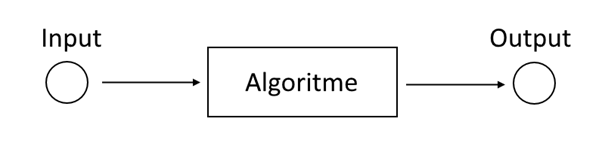
\includegraphics[width=\textwidth]{algorithm.png}
  \caption{Schematische weergave van een zelflerend systeeml}
  \label{fig:algorithm}
\end{figure}


Een zelflerend systeem is schematisch weergegeven in figuur \ref{fig:algorithm}. Bepaalde input data gaat het systeem en bepaalde output data komt uit het systeem. De input- en output data bestaat uit een getal, of uit meerdere getallen. Als de input bestaat uit een plaatje zal dit dus omgezet moeten worden in een reeks getallen om dit in een systeem te kunnen gebruiken.


\subsection{Trainen}
Een zelflerend systeem begint in de meeste gevallen zonder enige kennis. De gewenste \textbf{output} te kunnen produceren is het dus nodig om het systeem eerst input data te geven zodat het kan leren. Dit proces is wordt het “trainen” genoemd. Voor het trainen van een zelflerend systeem is training data nodig. Deze data moet gelijk of gelijkwaardig zijn aan de “echte” data. Deze training data kan in veel verschillende vormen voorkomen. De manier van trainen is afhankelijk van de vorm van de training data. Er zijn drie belangrijke manieren waarop een zelflerend systeem getraind kan worden: supervised, unsupervised en reinforcement learning.

\subsubsection{Supervised Learning}
In het geval van supervised learning heb je te maken met “labeled training data”. Ofwel van een bepaalde input is de gewenste output al bekend. Een klassiek voorbeeld van een “labeled data set” is een dataset van huisprijzen en huiseigenschappen (zie \ref{fig:labeled_dataset})
\label{fig:labeled_dataset}


\subsubsection{Unsupervised Learning}

\subsubsection{Reinforcement Learning}





\subsection{Evolutionary Systems}

\subsection{Conclusie}


\bibliography{references}
\bibliographystyle{plain}
